\documentclass[sigconf,screen,review]{acmart}

% --- Packages (acmart loads hyperref/url/cite/natbib internally - do NOT
%     reload them here, an option clash will follow). ---
\usepackage{amsmath,amssymb,amsfonts}
\usepackage{algorithm}
\usepackage{algpseudocode}
\usepackage{graphicx}
\usepackage{textcomp}
\usepackage{xcolor}
\usepackage{tikz}
\usetikzlibrary{arrows.meta,positioning,fit,backgrounds,shapes.geometric}
\usepackage{listings}
% booktabs is already loaded by acmart, but harmless to re-declare:
\usepackage{booktabs}
\usepackage[normalem]{ulem}

% --- Author-facing TODO macro (visible in PDF, easy to grep) ---
\newcommand{\todo}[1]{\textcolor{red}{\textbf{[TODO: #1]}}}

% --- Listing style ---
\lstset{
  basicstyle=\footnotesize\ttfamily,
  numbers=left, numberstyle=\tiny\color{gray}, numbersep=4pt,
  keywordstyle=\bfseries, commentstyle=\itshape\color{gray!70!black},
  showstringspaces=false, breaklines=true, frame=single, framerule=0.4pt,
  xleftmargin=10pt, xrightmargin=2pt, aboveskip=4pt, belowskip=4pt,
  morekeywords={for,each,if,then,else,return,let,select,one,exactly,end,procedure,Sniper}
}

% =============================================================================
% ACM rights / conference metadata. Most fields stay as \todo{} placeholders
% until camera-ready; \setcopyright should be confirmed against the ISSTA 2026
% author kit closer to the deadline.
% =============================================================================
\setcopyright{rightsretained}
\acmConference[ISSTA '26 Tool Demonstrations]{Proceedings of the 35th ACM SIGSOFT International Symposium on Software Testing and Analysis Tool Demonstrations}{October 3--9, 2026}{Oakland, CA, USA}
\acmBooktitle{Proceedings of the 35th ACM SIGSOFT International Symposium on Software Testing and Analysis Tool Demonstrations (ISSTA '26 Tool Demonstrations), October 3--9, 2026, Oakland, CA, USA}
\acmISBN{\todo{ISBN}}
\acmDOI{\todo{DOI}}
\acmPrice{15.00}
\acmYear{2026}
\copyrightyear{2026}

% --- ACM CCS (required, even if minimal) ---
\begin{CCSXML}
<ccs2012>
  <concept>
    <concept_id>10011007.10011074.10011099.10011102.10011103</concept_id>
    <concept_desc>Software and its engineering~Software testing and debugging</concept_desc>
    <concept_significance>500</concept_significance>
  </concept>
  <concept>
    <concept_id>10003033.10003079.10011704</concept_id>
    <concept_desc>Networks~Network services</concept_desc>
    <concept_significance>300</concept_significance>
  </concept>
</ccs2012>
\end{CCSXML}
\ccsdesc[500]{Software and its engineering~Software testing and debugging}
\ccsdesc[300]{Networks~Network services}

% --- Keywords ---
\keywords{REST API testing, microservices, distributed tracing, fault injection, large language models}

\begin{document}

\title{MIST: A Trace-Driven, LLM-Assisted Tool for Multi-Service REST API Test Generation}

% Single-blind track: author block is visible. Replace \todo{...} placeholders
% before submission.
\author{\todo{Author Name}}
\affiliation{%
  \institution{\todo{Institution}}
  \city{\todo{City}}
  \country{\todo{Country}}
}
\email{\todo{email@domain}}

\begin{abstract}
Microservice systems make REST API testing simultaneously more important and harder. Black-box test generators must reason about cross-service workflows that are not declared in any single OpenAPI specification, and the dominant ``HTTP 2xx is a pass'' oracle silently accepts soft errors that downstream services have already flagged. We present \textbf{MIST} (Microservice Integration \& Scenario Tester), an open-source tool that turns OpenTelemetry/Jaeger traces and OpenAPI specs into runnable, cross-service workflow tests. MIST is built around three named contributions: a \emph{Sniper Strategy} that injects exactly one fault at exactly one root API per negative variant so that any downstream anomaly is causally attributable, a \emph{Root API Mode} that exercises only entry-point APIs and observes internal behaviour through traces (avoiding state fabrication on internal endpoints), and a \emph{Trace-as-Oracle} layer that promotes span causality, error-status propagation, and soft-error patterns to checkable assertions. We bundle a TrainTicket \cite{Zhou2021TrainTicket} case study with a 10-fault injected-fault corpus and a public deployment, all reproducible from one properties file. Source code is at \url{https://github.com/miaoti/Rest/}. Screencast: \url{\todo{SCREENCAST-URL}}.
\end{abstract}

\maketitle


% =============================================================================
\section{Introduction}\label{sec:intro}

Microservice systems exchange business state across deeply coupled REST endpoints; testing that state from outside the system is now the bottleneck for black-box validation. Two gaps in the current generation of REST testing tools \cite{Arcuri2019EvoMasterTOSEM,MartinLopez2021RESTest,Atlidakis2019RESTler,HatfieldDodds2022Schemathesis,Liu2022MoRest,Kim2023ARATRL,Kim2024RESTGPT,Stennett2025AutoRestTest,Kim2025LlamaRestTest,Corradini2024DeepREST} stand out.

\textbf{Weak oracles.} The de facto oracle--the response status class--accepts as ``passing'' any 2xx body whose envelope contains \texttt{status:0, error:...}, a pattern endemic to enterprise REST APIs. Soft errors silently accumulate in test reports and never trigger a regression flag.

\textbf{State fabrication on internal endpoints.} Driving every API directly demands fabricating consistent state across many services. Generators that fall back to randomly-typed UUIDs end up exercising rejection paths instead of the intended business logic.

MIST addresses these gaps with three contributions, each implemented and shipped:

\begin{itemize}
  \item \textbf{Sniper Strategy}: every negative variant injects exactly one fault at exactly one root API, isolating the causal signal so downstream anomalies are attributable to a known mutation.
  \item \textbf{Root API Mode}: only entry-point APIs are exercised externally; the internal behaviour they trigger is observed through distributed traces, avoiding the state-fabrication problem.
  \item \textbf{Trace-as-Oracle}: span causality, error-status propagation, and soft-error patterns become first-class assertions that complement the response status class.
\end{itemize}

The artifact is open source at \url{https://github.com/miaoti/Rest/} and includes a TrainTicket \cite{Zhou2021TrainTicket} case study with a 10-fault injected-fault corpus reproducible from one properties file.

% =============================================================================
\section{Background and Motivating Example}\label{sec:bg}

Consider \texttt{POST /api/v1/adminroute\-ser\-vi\-ce/admin\-route} on TrainTicket, a request to create a route given a \texttt{startStation}, \texttt{endStation} and a \texttt{stationList}. On a sniper-mutated negative variant where the end station does not appear in the station list, the service replies \emph{HTTP 200 OK} along with the body
\begin{lstlisting}[basicstyle=\footnotesize\ttfamily,frame=none,numbers=none]
{"status":0,
 "msg":"start or end station not include in
        stationList.",
 "data":null}
\end{lstlisting}
A status-class oracle reports this run as a pass. The captured Jaeger trace (Figure~\ref{fig:trace}) shows that every span carries \texttt{http.status\_code=200} and no \texttt{otel.status\_code=ERROR} is set anywhere in the tree -- the network-level signals all confirm a clean 200. The only failure evidence lives in the response body, in the soft-error envelope (\texttt{status=0}, \texttt{data=null}). A trace-aware oracle that learns and caches per-API body-pattern rules catches this; it also reads off the trace which service rejected the request (\texttt{ts-admin-route-service}). This is exactly the situation MIST is built for.

% =============================================================================
\section{Tool Overview and Architecture}\label{sec:arch}

\begin{figure*}[t]
  \centering
  % Figure 1: MIST architecture.  Polished sigconf-friendly version.
% Pipeline of five components + SUT cluster + run output.  Inputs are
% described in the caption, not drawn on the canvas, so no input-feed
% wires can clip box text.
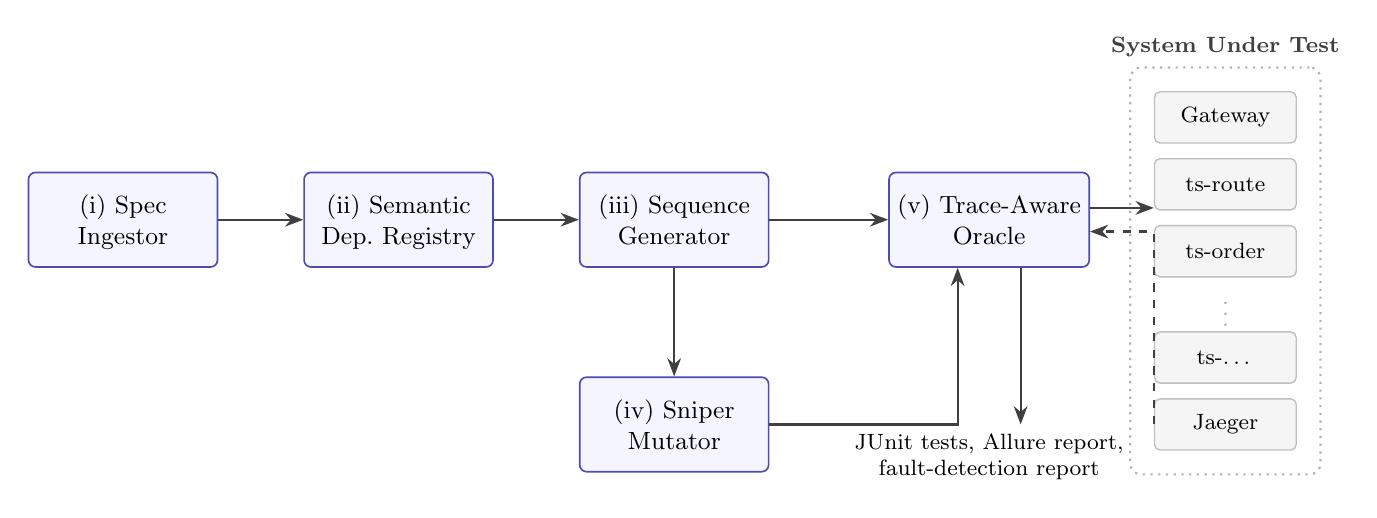
\begin{tikzpicture}[
    font=\small,
    >={Stealth[length=2.4mm]},
    comp/.style    ={draw=blue!40!gray, line width=0.6pt, rounded corners=2.5pt,
                     fill=blue!4, minimum height=12mm, minimum width=24mm,
                     align=center, inner sep=3pt, text depth=0pt},
    sut/.style     ={draw=gray!50, line width=0.5pt, rounded corners=2pt,
                     fill=gray!8, minimum height=6.5mm, minimum width=18mm,
                     align=center, inner sep=2pt, font=\footnotesize},
    sutgap/.style  ={align=center, inner sep=1pt, font=\footnotesize\itshape,
                     text=gray!70},
    outlbl/.style  ={font=\footnotesize, align=center, anchor=north},
    flow/.style    ={->, thick, >=Stealth, draw=black!75},
    backflow/.style={->, thick, dashed, >=Stealth, draw=black!75}
]

% --- Four components on the main row at y=0. ---
\node[comp] (ingest)   at ( 0.0, 0)   {(i) Spec\\Ingestor};
\node[comp] (registry) at ( 3.5, 0)   {(ii) Semantic\\Dep.\ Registry};
\node[comp] (gen)      at ( 7.0, 0)   {(iii) Sequence\\Generator};
\node[comp] (oracle)   at (11.0, 0)   {(v) Trace-Aware\\Oracle};
\node[comp] (mut)      at ( 7.0,-2.6) {(iv) Sniper\\Mutator};

% --- System Under Test cluster.  Explicit 'ts-...' row between named
%     services so the figure tells the reader 'these two are
%     representative of many'. ---
\node[sut]   (gw)   at (14.0, 1.30)  {Gateway};
\node[sut]   (svc1) at (14.0, 0.45)  {ts-route};
\node[sut]   (svc2) at (14.0,-0.40)  {ts-order};
\node[sutgap](dots) at (14.0,-1.10)  {$\vdots$};
\node[sut]   (svcn) at (14.0,-1.75)  {ts-\dots};
\node[sut]   (jgr)  at (14.0,-2.60)  {Jaeger};

\begin{scope}[on background layer]
  \node[draw=gray!60, dotted, thick, rounded corners=4pt, inner sep=3mm,
        fit=(gw)(jgr),
        label={[font=\footnotesize\bfseries, gray!50!black]above:System Under Test}] {};
\end{scope}

% --- Run output below the oracle, offset right of the mut->oracle wire. ---
\node[outlbl] (out) at (11.0,-2.6)
  {JUnit tests, Allure report,\\fault-detection report};

% --- Main horizontal pipeline. ---
\draw[flow] (ingest)   -- (registry);
\draw[flow] (registry) -- (gen);
\draw[flow] (gen)      -- (oracle);

% --- Generator -> Sniper Mutator (clean vertical). ---
\draw[flow] (gen.south) -- (mut.north);

% --- Sniper Mutator -> Oracle. ---
\draw[flow] (mut.east) -| ([xshift=-4mm]oracle.south);

% --- Oracle <-> SUT.  Two parallel arrows distinguished by +/- 1.5mm y-shift. ---
\draw[flow]     ([yshift= 1.5mm]oracle.east)
            -- ([yshift= 1.5mm]oracle.east -| gw.west);
\draw[backflow] (jgr.west)
            -- ([yshift=-1.5mm]oracle.east -| jgr.west)
            -- ([yshift=-1.5mm]oracle.east);

% --- Oracle -> output (drops straight down, offset right of mut->oracle). ---
\draw[flow] ([xshift=4mm]oracle.south) -- ([xshift=4mm]oracle.south |- out.north);

\end{tikzpicture}

  \caption{MIST architecture. Five components are arranged left-to-right by data flow; the dotted box is the System Under Test. Solid arrows are HTTP requests issued by MIST; the dashed arrow is the Jaeger trace pulled back per step by the Trace-Aware Oracle.}
  \label{fig:arch}
\end{figure*}

Figure~\ref{fig:arch} shows the five components. All numbers in this paper come from a MIST run against the bundled TrainTicket deployment described in Section~\ref{sec:case}.

\textbf{(i) Spec Ingestor.} Parses an OpenAPI specification --- obtained from the SUT operator or aggregated from per-service \texttt{/v3/api-docs} endpoints --- and emits a multi-service test configuration. The bundled TrainTicket spec contains 265 operations across 37 REST-exposed services, defining MIST's test scope. Components without a discoverable HTTP surface (asynchronous workers, message brokers, internal-only RPC services) lie outside any black-box tool's reach by construction.

\textbf{(ii) Semantic Dependency Registry with JIT Binding.} A producer/consumer index over the spec records, for every parameter whose name ends in \texttt{Id}/\texttt{ID}/\texttt{uuid}, the API and JSON path that historically produces it. At generation time the registry's \texttt{findProducer} call returns a \texttt{ProducerBinding} that the Sequence Generator wires \emph{just-in-time}, so a value computed at runtime by an earlier step in the same scenario is plugged into the right field of a later step.

\textbf{(iii) Sequence Generator (Root API Mode).} Mines workflow scenarios from Jaeger traces through a five-phase pipeline: cross-trace data-dependency merging, session/time-window merging, single-root deduplication, weakly-connected-component shattering on the dependency graph, and missing-baseline decomposition. With Root API Mode enabled (\texttt{mst.gener\-ate.only.first.step=true}, the default) the generator preserves all gateway-entry calls in a scenario but prunes internal step-API spans, since those are observed through the trace rather than driven directly. A scenario with three root calls produces a 3-step JUnit test.

\textbf{(iv) Sniper Mutator.} Builds an \texttt{InvalidInputPool} per parameter, drawing from eight schema-aware fault categories (TYPE\_MISMATCH, REGEX\_MISMATCH, SEMANTIC\_MISMATCH, OVERFLOW, EMPTY/NULL, SPECIAL\_CHARACTERS, BOUNDARY\_VIOLATION). For every negative variant it picks exactly one parameter at exactly one root call and exactly one fault value (Section~\ref{sec:sniper}).

\textbf{(v) Trace-Aware Oracle.} Each emitted JUnit test, after firing a request, fetches the corresponding Jaeger trace and evaluates four assertion families: HTTP status class, response-body soft-error pattern (LLM-inferred rule cached per API), span error-status propagation, and root-cause matching against the injected-fault registry.

% =============================================================================
\section{Core Innovations}\label{sec:innov}

The three contributions interlock. The Sniper Strategy's single-fault discipline is what makes Trace-as-Oracle's downstream signals causally interpretable; Root API Mode's external-only driving is what allows traces to be the primary oracle without confounding from direct internal calls. None of the three could close the oracle and state-fabrication gaps alone; the combination is what does.

\subsection{Sniper Strategy}\label{sec:sniper}

A negative test that mutates several parameters at once leaves the oracle unable to attribute any observed downstream anomaly to a specific cause; symmetrically, a single-fault test on a non-root call cannot be reasoned about either, because the trace prefix is itself driven by other, possibly mutated values. The Sniper Strategy isolates cause from effect by tightening both axes at once.

\begin{algorithm}[H]
\caption{Sniper Strategy (per negative variant)}\label{alg:sniper}
\begin{algorithmic}[1]
\Procedure{Sniper}{$scenario, params, pools$}
  \State $r \gets$ the first root call in $scenario$
  \State $p \gets$ select one parameter from $params(r)$ via round-robin
  \State $c \gets$ select one applicable fault category for $p$'s schema
  \State $v \gets pools[r][p][c].\text{nextRoundRobin}()$
  \State \textbf{lock} parameter $p$ on root $r$ to value $v$
  \State all other parameters on $r$ and all later roots are filled
  \Statex \quad\quad from positive sources (shared pool, smart fetch, JIT bind)
  \State \textbf{record} $(r, p, c, v)$ on the test case as the fault target
  \State \Return rendered \texttt{MultiServiceTestCase}
\EndProcedure
\end{algorithmic}
\end{algorithm}

The schema-applicability filter (\texttt{InvalidInputType.appliesTo}) drops nonsense combinations: a boolean parameter never receives a 5000-character OVERFLOW payload labelled OVERFLOW, because the value would actually be a TYPE\_MISMATCH wearing the wrong label. Round-robin scheduling guarantees coverage breadth: each parameter is targeted with each applicable category before any combination repeats. The pre-recorded \texttt{(r,p,c,v)} tuple flows straight into the fault-detection report so every observed failure is attributable to one specific mutation.

Compared with conventional black-box fuzzing where multiple parameter mutations interact \cite{Arcuri2019EvoMasterTOSEM,Atlidakis2019RESTler,HatfieldDodds2022Schemathesis}, the Sniper Strategy trades exhaustive combinatorial coverage for causal attributability--the property that makes the trace-aware oracle's downstream signals interpretable.

\subsection{Root API Mode}\label{sec:rootmode}

Internal microservice endpoints typically presuppose state that can only be created through specific upstream calls (an \texttt{orderId} that exists in the database, a session whose token has not expired, a route that has stations). Black-box generators that drive those endpoints directly must fabricate the state, and a fabrication failure looks identical to a real test failure.

Root API Mode bypasses the problem. The generator extracts only the \emph{root} API calls from each Jaeger scenario--the gateway-entry HTTP spans that have no HTTP parent--and replays only those externally. The internal behaviour they trigger is observed through the captured trace, not driven. Concretely, the writer emits one JUnit step per root call, and an attached Jaeger fetch reads back the full causal subtree.

The mode is one boolean (\texttt{mst.gener\-ate.only.first.step}, default \texttt{true}). Disabling it falls back to a multi-step replay where every internal HTTP span also becomes a step. This paper reports only the root-only mode.

\subsection{Trace-as-Oracle}\label{sec:traceoracle}

\begin{figure*}[t]
  \centering
  % Figure 2: Real captured Jaeger trace from a Sniper negative variant
% against POST /api/v1/adminrouteservice/adminroute on TrainTicket.
% Trace ID: d4c577d47bcba04a00ef9b3edcbcacf6 (test_negative_POST_1_81).
% Source: src/main/resources/My-Example/trainticket/allure-results/
%         4a67e7c8-4fd2-4b6a-a698-1b1cec487a6d-attachment.txt
%
% Layout: 5-span parent-child cascade on the top, Trace-Aware Oracle
% verdict in prose underneath.  Designed to fit acmart sigconf full
% width (figure*) with the 'review' line-number gutters subtracted
% from the usable canvas.
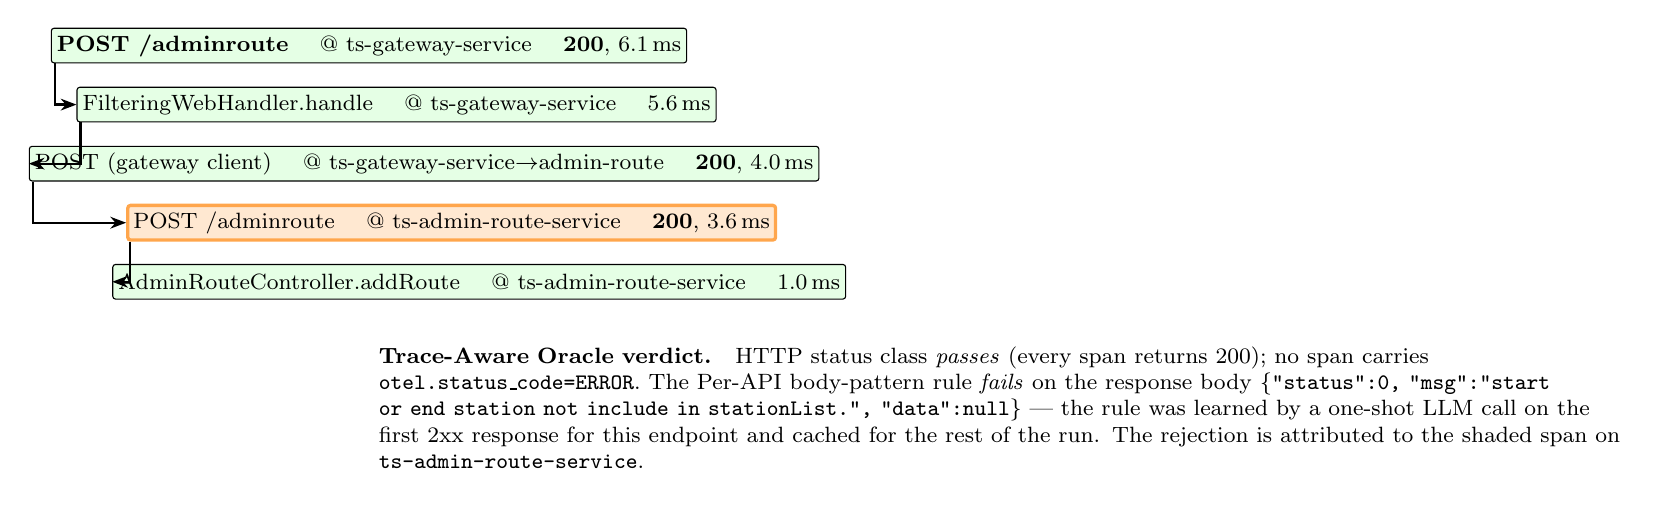
\begin{tikzpicture}[
    font=\footnotesize,
    >={Stealth[length=2mm]},
    span/.style={draw, rounded corners=1pt, minimum height=4.4mm,
                 align=left, inner sep=2pt, font=\footnotesize},
    spanok/.style={span, fill=green!10},
    spansoft/.style={span, fill=orange!18, draw=orange!70, very thick},
    edge/.style={->, thick}
]

% --- Spans: indented cascade, parent -> child ---
\node[spanok]  (s1) at (0.00, 0)
  {\textbf{POST /adminroute} \quad @ ts-gateway-service \quad \textbf{200}, 6.1\,ms};
\node[spanok]  (s2) at (0.35,-0.75)
  {FilteringWebHandler.handle \quad @ ts-gateway-service \quad 5.6\,ms};
\node[spanok]  (s3) at (0.70,-1.50)
  {POST (gateway client) \quad @ ts-gateway-service$\to$admin-route \quad \textbf{200}, 4.0\,ms};
\node[spansoft](s4) at (1.05,-2.25)
  {POST /adminroute \quad @ ts-admin-route-service \quad \textbf{200}, 3.6\,ms};
\node[spanok]  (s5) at (1.40,-3.00)
  {AdminRouteController.addRoute \quad @ ts-admin-route-service \quad 1.0\,ms};

% Parent-child arrows
\draw[edge] (s1.south west) ++(0.05,0) |- (s2.west);
\draw[edge] (s2.south west) ++(0.05,0) |- (s3.west);
\draw[edge] (s3.south west) ++(0.05,0) |- (s4.west);
\draw[edge] (s4.south west) ++(0.05,0) |- (s5.west);

% --- Trace-Aware Oracle verdict, in prose, below the trace ---
\node[align=left, anchor=north west, font=\footnotesize, text width=16cm]
  at (0,-3.7) {%
    \textbf{Trace-Aware Oracle verdict.}\quad
    HTTP status class \emph{passes} (every span returns 200);
    no span carries \texttt{otel.status\_code=ERROR}.
    The Per-API body-pattern rule \emph{fails} on the response body
    \texttt{\{"status":0, "msg":"start or end station not include in stationList.", "data":null\}}
    --- the rule was learned by a one-shot LLM call on the first 2xx response for this endpoint
    and cached for the rest of the run.
    The rejection is attributed to the shaded span on \texttt{ts-admin-route-service}.%
  };

\end{tikzpicture}

  \caption{Real captured Jaeger trace from a MIST sniper-mutated negative variant against \texttt{POST /api/v1/admin\-route\-ser\-vice/admin\-route} on TrainTicket (trace ID \texttt{d4c577d4\dots\,acf6}; source: this repository's Allure attachments). Every span carries \texttt{http.status\_code=200} and no \texttt{otel.status\_code=ERROR} is set --- the network-level oracles all pass. The Trace-Aware Oracle catches the failure through the cached per-API body-pattern rule, and uses the trace to attribute the rejection to \texttt{ts-admin-route-service}.}
  \label{fig:trace}
\end{figure*}

Figure~\ref{fig:trace} renders an actual trace from the repository's captured Allure attachments. The HTTP-status-class oracle, on its own, would only see ``200 OK on the root call'' and pass the test. The Trace-Aware Oracle additionally evaluates:
\begin{itemize}
  \item span causality (does the trace tree match the structural pattern derived from the original recorded scenario?),
  \item error-status propagation (no descendant carries \texttt{otel.status\_code=ERROR} or \texttt{http.status\_code} $\geq 400$),
  \item LLM-inferred soft-error rules cached per API in \texttt{target/soft-error-rule-cache.json}, so that envelope-level signals such as \texttt{status:0} are recognised on the very first 2xx response and reused thereafter without further LLM calls,
  \item root-cause matching of the response \texttt{faultName} against the injected-fault registry.
\end{itemize}

The cache makes the LLM cost bounded: roughly two calls per distinct API regardless of how many tests touch that API.

% =============================================================================
\section{Usage Scenarios and Case Study}\label{sec:case}

\subsection{Scenario A: targeted regression after a change}

A developer changes the \texttt{ts-admin-route-service} input validation. The relevant scenarios are already mined; a single re-run with \texttt{faulty.ratio=0.8} re-exercises the service with the same Sniper-tightened negative variants and surfaces any regression in the fault-detection report:
\begin{lstlisting}[basicstyle=\footnotesize\ttfamily,frame=none,numbers=none]
$ java -jar target/restest.jar \
   src/main/resources/My-Example/trainticket-demo.properties
\end{lstlisting}

\subsection{Scenario B: exploratory fault detection across the system}

A QA engineer runs the bundled demo end-to-end. The configuration emits and executes 2733 test cases\footnote{Variant count from a representative MIST run on the bundled deployment, fault-detection report \texttt{trainticket\_twostage\_test\_1778039778981}.} on the deployed TrainTicket against the 10-fault injected-fault corpus described in \texttt{INJECTED\_FAULTS.md}. End-to-end wall-clock time is approximately 20\,h, of which roughly 12\,h is LLM (DeepSeek \texttt{deepseek-chat}) inference latency. The bulk of LLM cost is positive-input synthesis (one prompt per parameter per variant under \texttt{tests\-per\-oper\-a\-tion=100}); the soft-error rule cache contributes a one-time $\sim$2 prompts per distinct API and is amortised across the run. The remaining $\sim$8\,h covers scenario extraction, variant generation, JUnit emission, in-process execution, and trace-aware oracle evaluation.

Table~\ref{tab:faults} reports detection on the most recent end-to-end run. All ten injected faults are detected.

\begin{table}[t]
\centering
\caption{TrainTicket 10-fault injected-fault corpus, detection on the most recent end-to-end MIST run.}
\label{tab:faults}
\footnotesize
\begin{tabular}{@{}llcl@{}}
\toprule
\textbf{Fault ID} & \textbf{Description} & \textbf{Det.} & \textbf{Mechanism} \\
\midrule
\textsc{Insufficient\_Stations} & route has $<2$ stations & \checkmark & \todo{mech} \\
\textsc{Invalid\_Station\_Name\_Length} & station name out of [2,50] & \checkmark & \todo{mech} \\
\textsc{Invalid\_Contacts\_Name} & numeric/empty contact name & \checkmark & \todo{mech} \\
\textsc{Invalid\_Seat\_Number} & seat $\not\sim$ \texttt{\textbackslash d+[A-Z]} & \checkmark & \todo{mech} \\
\textsc{Invalid\_Price\_Rate} & non-positive price rate & \checkmark & \todo{mech} \\
\textsc{Invalid\_Route\_Id} & empty \texttt{routeId} & \checkmark & \todo{mech} \\
\textsc{Invalid\_Station\_Name} & empty start/end place & \checkmark & \todo{mech} \\
\textsc{Invalid\_Station\_Length} & station name length $\notin[2,50]$ & \checkmark & \todo{mech} \\
\textsc{Invalid\_Trip\_Id\_Format} & empty/whitespace \texttt{tripId} & \checkmark & \todo{mech} \\
\textsc{Invalid\_Trip\_Id\_Length} & \texttt{tripId} length $\notin[4,20]$ & \checkmark & \todo{mech} \\
\bottomrule
\end{tabular}
\end{table}

The mechanism column is to be filled per-row from the most-current fault detection report (see \texttt{NOTES\_TO\_AUTHOR.md}, Q2). Four mechanism kinds are recognised: HTTP $\geq 4xx$, LLM soft-error rule, Jaeger error span, and injected-fault registry match.

% =============================================================================
\section{Related Work and Conclusion}\label{sec:rw}

\textbf{REST API testing.} EvoMaster \cite{Arcuri2017EvoMaster,Arcuri2019EvoMasterTOSEM} pioneered evolutionary search-based test generation; RESTest \cite{MartinLopez2021RESTest}, on which MIST is built, contributed the constraint-based and ART generators. Related schema-driven, feedback-guided, and LLM-integrated generators \cite{Atlidakis2019RESTler,HatfieldDodds2022Schemathesis,Liu2022MoRest,Kim2023ARATRL,Corradini2024DeepREST,Kim2024RESTGPT,Kim2025LlamaRestTest,Stennett2025AutoRestTest} target single-service APIs and use status-class oracles, not cross-service trace-as-oracle reasoning.

\textbf{Trace-based testing.} Distributed tracing originates with Dapper \cite{Sigelman2010Dapper}; OpenTelemetry \cite{OpenTelemetry} and Jaeger \cite{Jaeger} are the contemporary open standards. The TrainTicket benchmark \cite{Zhou2021TrainTicket} is the canonical microservice testbed and ships with documented fault patterns. To our knowledge, MIST is the first openly available REST API testing tool that mines workflow scenarios from production traces and uses span-level evidence as a primary oracle.

\textbf{Conclusion.} MIST closes two oracle and state-fabrication gaps that are particularly painful in microservice REST APIs: it sniper-mutates one root API per variant, observes downstream behaviour through traces rather than driving internal endpoints, and elevates trace-derived properties to checkable assertions. The artifact, the TrainTicket case study, and the 10-fault corpus are open at \url{https://github.com/miaoti/Rest/}.



% =============================================================================
\section{Tool Availability}\label{sec:avail}

MIST is open-source and available at \url{https://github.com/miaoti/Rest/}, with documentation covering installation, configuration, and a TrainTicket walkthrough. A screencast demonstrating MIST on the TrainTicket benchmark is at \url{\todo{SCREENCAST-URL}}. The archived snapshot used in this paper is available at \url{\todo{ZENODO-DOI}}.

\textbf{Data Availability.} All artifacts referenced in this paper --- the MIST source code, the TrainTicket merged OpenAPI specification, the 10-fault injection registry, captured Jaeger traces, and fault-detection reports --- are included in the public repository and the Zenodo snapshot.

\bibliographystyle{ACM-Reference-Format}
\bibliography{refs}

\end{document}
